\chapter{Stany}

Ten rozdział opisuje stany postaci gracza i obiektów fauny (rys 4.1, 4.2).

\section{Stany postaci gracza}

Przy rozpoczęciu nowej rozgrywki lub wczytaniu jej tworzony będzie obiekt postaci gracza. Po inicjalizacji przejdzie do stanu pasywnego. W tym stanie postać gracza nie będzie wykonywać żadnych akcji. 

Po naciśnięciu któregoś z przycisków ruchu postać przejdzie do stanu ruchu. Jeżeli postać będzie w stanie pasywnym lub ruchu i naciśnięty zostanie przycisk skoku, to postać przejdzie do stanu skoku. Jeżeli w tym stanie postać dotknie ziemi i klawisz skoku nie będzie wciśnięty, to postać przejdzie do stanu spoczynku (jeżeli żaden z przycisków ruchu nie będzie wciśnięty) lub do stanu ruchu (jeżeli którykolwiek z przycisków ruchu będzie wciśnięty). 

Jeżeli postać będzie w stanie spoczynku i akcja skanowania będzie możliwa (kamera skierowana na obiekt flory i fauny, którego typu żaden inny obiekt nie został zeskanowany, i będzie to obiekt najbliższy graczowi) to, gdy gracz wciśnie przycisk skanowania, postać przejdzie do stanu skanowania. Postać wyjdzie ze stanu skanowania jeżeli gracz puści przycisk skanowania lub akcja skanowania przestanie być możliwa. 

Jeżeli postać będzie w stanie spoczynku i akcja zbierania będzie możliwa (kamera skierowana na obiekt flory, fauny lub terenu, który może zostać zebrany, i będzie to obiekt najbliższy graczowi), to gdy gracz wciśnie przycisk skanowania, postać przejdzie do stanu skanowania. Postać wyjdzie ze stanu skanowania jeżeli gracz puści przycisk skanowania lub akcja skanowania przestanie być możliwa. 

Jeżeli postać będzie w stanie spoczynku i gracz otworzy menu budowania to postać przejdzie do stanu budowania. Gdy gracz zamknie menu budowania to postać przejdzie ze stanu budowania do stanu pasywnego.

\begin{figure}[H]
    \centering
        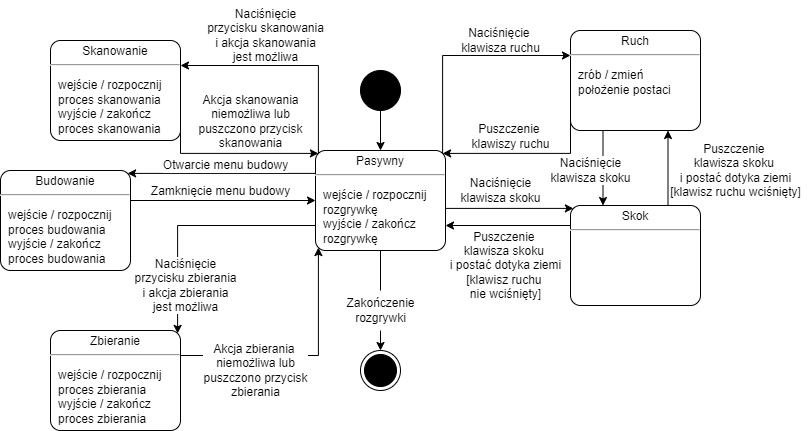
\includegraphics[width = 0.97\textwidth]{postac_stany.png}
        \index{Diagram stanów postaci}
        \caption{Diagram stanów postaci}
\end{figure}

\section{Stany zwierząt}

Po stworzeniu obiektu znajdzie się on w stanu przyjaznym, w którym posiadać będzie zachowania, które nie będą agresywne względem postaci gracza. Gdy nastanie noc, obiekt zwierzęcia przejdzie do stanu wrogiego. W tym stanie posiadać będzie wrogie zachowania. Będzie atakować gracza i dążyć do zmniejszenia jego wskaźnika życia do zera. Gdy nastanie dzień, obiekt zwierzęcia powróci do stanu przyjaznego.

Jeżeli gracz zmniejszy wskaźnik życia zwierzęcia do zera, zwierzę przejdzie do stanu zabitego. W tym stanie straci wszelkie zachowania. Gracz będzie mógł zeskanować obiekt w takim stanie. Jeżeli gracz zbierze surowce z zabitego zwierzęcia, obiekt zwierzęcia zostanie usunięty. 

\begin{figure}[H]
    \centering
        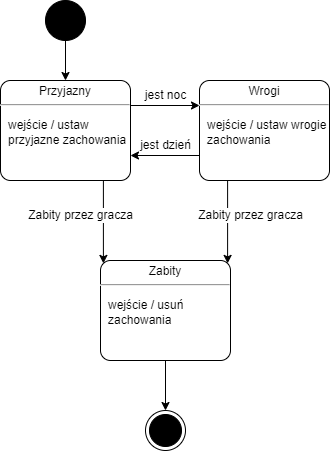
\includegraphics[width = 0.5\textwidth]{stany_fauny.png}
         \index{Diagram stanów zwierząt}
         \caption{Diagram stanów zwierząt}
\end{figure}